% !TeX root = ../thuthesis-example.tex

\chapter{研究背景}
\label{background}
在机器人学研究中,视觉惯性测距(VIO)在导航、定位和感知任务中发挥着举足轻重的作用。VIO 系统通过融合来自视觉和惯性传感器的数据来估计机器人的姿态(位置和方向)。近年来,人们提出了许多 VIO 方法,例如直接使用像素强度估算摄像机运动的直接方法,以及基于特征的方法等。其中,基于特征的方法使用图像特征(点、线或平面)来估计传感器位姿和周围环境的地图。
\begin{figure}
  \centering
  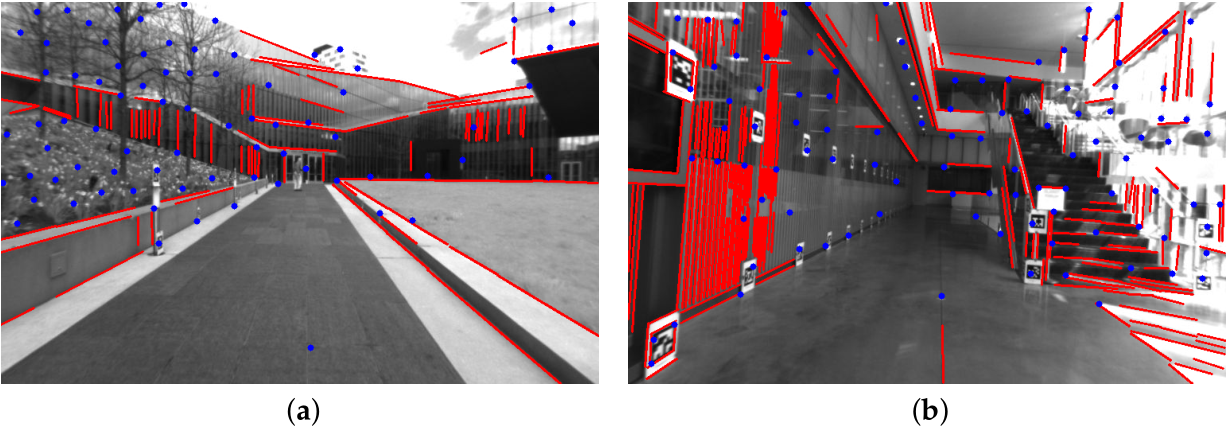
\includegraphics[width = 0.75\textwidth]{plbg.png}
  \caption{图像中的点线特征}
  \label{fig_plbg}
\end{figure}
基于点的 VIO 算法发展最为成熟,现有点VIO算法在精度和速度方面都表现出了卓越的性能,可以应用于需要实时跟踪的场景。然而,在低纹理环境或重复纹理环境中(例如走廊、道路、开阔水域等),由于点特征信息匮乏,基于点的 VIO 算法会出现性能下降的问题。为了利用环境中丰富的边缘信息,克服点信息失效的问题,研究人员进一步开发了基于线特征的VIO算法,并将线特征作为辅助构建了点线联合的VIO框架,现有框架包括PL-SLAM\cite{pumarola2017pl},PL-VINS\cite{fu2020pl}等。但是,由于线特征存在参数化复杂且耗时的问题,现有的点线联合VIO框架难以在嵌入式设备上实时运行,使得线特征的精度增益难以在小型无人设备(比如无人机)上得到实现。 为了构建一个可以在嵌入式小型无人设备上实时运行的点线VIO系统,本工作首先基于神经网络的特征推理网络,提出了点线融合的SP-SOLD2网络,并利用自监督训练使得该网络可以通过一次推理得到特征点、特征线以及同时适用于点线匹配的描述子;为了将各类点线提取和匹配方法灵活应用于VIO任务中,本工作构建了一个前端方法可自定义的NN-PL-VIO框架,并利用SP-SOLD2点线联合网络以及一系列速度优化方法,得到了一个可以在嵌入式设备Orin NX上实时运行的点线联合VIO系统。

\section{点特征提取及描述方法}
点特征提取方法可以简单地分类为传统方法和深度学习方法两大类,其中传统方法是通过一系列数学计算得到特征点及其描述子,具有数学可解释性;而深度学习方法则是通过设计网络来端到端推理定位特征点,和描述子可以不耦合。一些常见的传统点特征方法如下:
\begin{enumerate}
  \item Harris角点检测算法(Harris Corner Detection):该算法通过计算图像中每个像素点的角点响应函数来检测角点。角点响应函数基于图像中局部区域的亮度变化,对角点位置具有较高的响应值。Harris角点检测算法具有旋转不变性和一定程度的尺度不变性。
  \item Shi-Tomasi角点检测算法(Shi-Tomasi Corner Detection):该算法是对Harris角点检测算法的改进。它使用了一个更加鲁棒的角点响应函数,能够在保持高角点检测率的同时提供更好的角点定位精度。
  \item SIFT(尺度不变特征变换,Scale-Invariant Feature Transform):SIFT是一种广泛应用的特征点提取算法,能够在不同尺度和旋转条件下提取稳定的特征点。SIFT算法通过在图像中检测局部极值点,并在多个尺度上计算尺度空间特征向量,得到具有尺度不变性的特征描述子。
  \item SURF(加速稳健特征,Speeded-Up Robust Features):SURF算法是对SIFT算法的改进,通过提出一种快速的特征点检测和描述子计算方法,实现了更高的计算效率。SURF算法利用图像的Hessian矩阵来检测特征点,并使用Haar小波响应描述子来描述特征。
  \item FAST(Features from Accelerated Segment Test):FAST算法是一种快速的角点检测算法,适用于实时应用。该算法基于像素灰度值的变化来检测角点,通过高效的特征点筛选策略提高了检测速度。
  \item ORB(Oriented FAST and Rotated BRIEF):ORB算法是对FAST和BRIEF(Binary Robust Independent Elementary Features)算法的结合。它在FAST算法的基础上引入了旋转不变性,并使用二进制描述子来进行特征匹配,具有较高的计算效率和良好的性能。
\end{enumerate}
而基于神经网络的点特征提取方法可以分为两种类别:检测和描述分离的方法与端到端匹配的方法。其中检测和描述分离的方法是设计两个网络或者一个联合网络,分别进行点特征的检测和点描述子的提取;而端到端匹配的方法则是直接设计和训练一个网络,此网络可以接受两个输入图像,直接给出特征匹配结果。基于神经网络的方法总结如表\ref{tab_NNPoint}:
\begin{table}[!ht]
  \centering
  \begin{tabular}{|c|c|c|}
  \hline
      名称 & 类型 & 描述 \\ \hline
      ASLFeat\cite{luo2020aslfeat} & 点检测 & \parbox[c][16ex]{7cm}{使用可变形卷积网络,利用固有的特征层次,提出了一种多级检测机制,该机制不仅在没有额外学习权重的情况下可以恢复低层细节以进行精确的关键点定位} \\ \hline
      SuperPoint\cite{detone2018superpoint} & 点检测和描述子提取联合 & \parbox[c][13ex]{7cm}{介绍了一个自监督框架,利用运行在全尺寸图像上的全卷积模型,在一个前向传递中同时计算像素级兴趣点位置和关联描述子} \\ \hline
      R2D2\cite{revaud2019r2d2} & 点检测和描述子提取联合 & \parbox[c][13ex]{7cm}{在D2-Net基础上考虑了特征检测的可重复性和可靠性,为检测得分设计了损失函数,使用全卷积网络推理特征点及其描述子} \\ \hline
      LoFTR\cite{sun2021loftr} & 端到端匹配 &\parbox[c][13ex]{7cm}{ 使用了Transformer中的自我和交叉注意力层(self and cross attention layers)来获取两个图像的特征描述符,实现无检测器的局部特征匹配。} \\ \hline
      Patch2Pix\cite{zhou2021patch2pix} & 端到端匹配 & \parbox[c][16ex]{7cm}{建立了一种新的匹配细化网络,首先得到 patch-level 的匹配,再细化到 pixel-level 的匹配,网络可以同时细化匹配并排除错误匹配,且训练不需要像素级的 GT 对应关系。} \\ \hline
      SuperGlue\cite{sarlin2020superglue} & 描述子提取 & \parbox[c][16ex]{7cm}{提出了一种能够同时进行特征匹配以及滤除外点的网络,基于注意力机制提出了一种灵活的内容聚合机制,这其能够同时感知潜在的3D场景以及进行特征匹配。} \\ \hline
  \end{tabular}
  \caption{基于神经网络的点特征提取方法}
  \label{tab_NNPoint}
\end{table}

\section{线特征提取描述方法}
线特征的提取方法可以分为三种类别:基于全局哈夫的方法、基于局部信息的方法,以及基于深度学习的方法,下面将分别介绍。
\subsection{基于全局哈夫的方法}
基于任何一个点都可能是线上的点的假设,此方法对所有点按照下式进行Hough变换:
\[
  \rho = x_0\cos{\theta}+y_0\sin{\theta}
\]
则一个点$(x_0,y_0)$将对应Hough平面下的一系列曲线;Hough平面上产生交点的曲线,则对应原平面上同线的一系列点,如图\ref{fig_hough}所示。
\begin{figure}
  \centering
  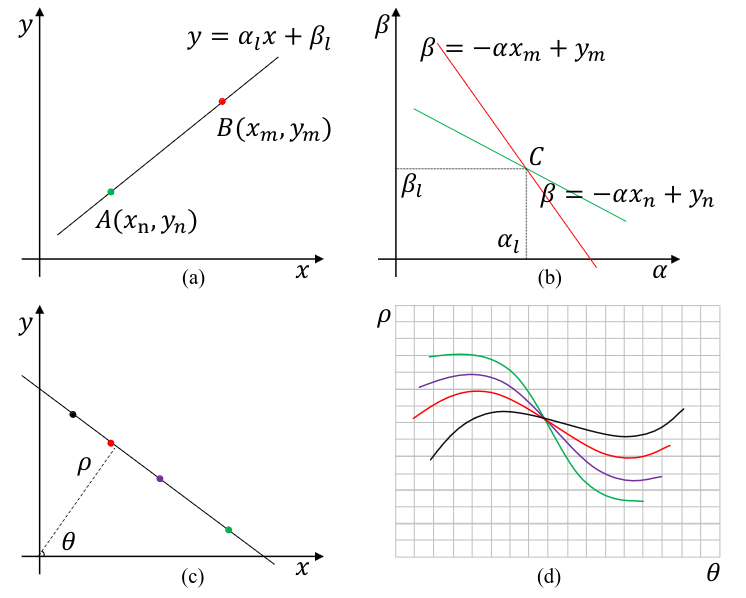
\includegraphics[width = 0.75\textwidth]{hough.png}
  \caption{哈夫变换示意图}
  \label{fig_hough}
\end{figure}
利用Hough变换,此方法利用严格的数学推导得到共线点关系,但是作为一个全局方法,需要对所有像素进行操作(包括预处理和变换),复杂度较高,并且空间定量搜索方式提取的数量和质量一般,不能定位线段端点。

\subsection{基于局部信息的方法}
此类方法利用局部信息(图像梯度和边缘检测结果等)探寻可能存在线段的位置,提取线段。LSD\cite{von2008lsd}是一种典型的基于局部信息的线段提取方法,如图\ref{fig_LSD}所示。该算法首先对输入图像进行多尺度的高斯滤波,以便检测不同尺度下的线段。接着,LSD会计算图像的梯度信息,找出梯度变化显著的区域,作为线段潜在区域。然后,通过区域合并方法,相邻的梯度变化显著的像素点会被组合成候选线段,计算线段位置、长度、方向和梯度等参数。为了去除冗余线段,LSD在最后会使用非极大值抑制和滤波的方法来筛选得到最终的线段提取结果。
\begin{figure}
  \centering
  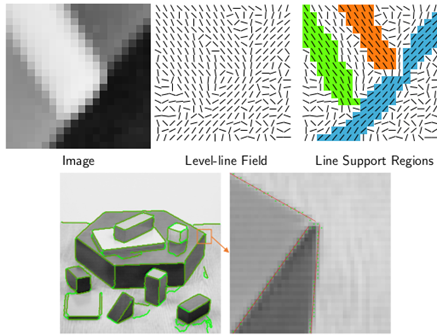
\includegraphics[width = 0.75\textwidth]{LSD.png}
  \caption{LSD线提取方法}
  \label{fig_LSD}
\end{figure}
基于局部信息的方法虽然一定程度上降低了线段提取的复杂度,但是算法仍为像素级操作,空间复杂度高,并且缺乏语义和全局约束信息,此类方法易受到噪声干扰。

\subsection{基于深度学习的方法}
基于深度学习的线段提取方法利用神经网络来自动检测和提取图像中的线段,能够通过网络设计更灵活地融合全局和局部信息,得到准确度和实用性更好的线段提取结果。根据网络设计的思路,可以分为Top-Down策略、Bottom-Up策略和Tri-Point策略。
\begin{figure}
  \centering
  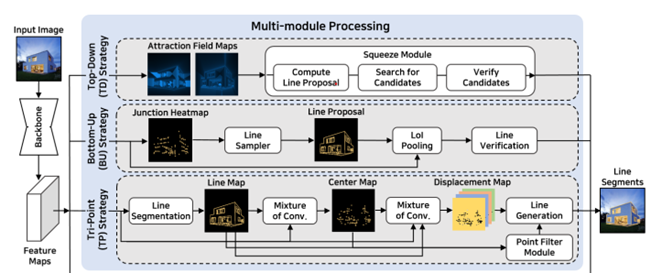
\includegraphics[width = 0.75\textwidth]{DL.png}
  \caption{基于深度学习的线特征提取方法}
  \label{fig_DL}
\end{figure}
\begin{enumerate}
  \item Top-Down策略:自上而下的策略核心是从线段可能存在的区域“挤压”得到线段提取结果,故而网络提取的目标是与线段相关的概率图。
  \item Bottom-Up策略:自下而上的策略核心是先找到线段的端点,再从端点定位线段。
  \item Tri-Point策略:Tri-Point策略核心是定位线上的某些点,用多个点和线段之间的距离关系定位线段。
\end{enumerate}

线提取方法总结如表\ref{tab_Line}所示:
\begin{table}[!ht]
  \centering
  \begin{tabular}{|c|c|c|c|c|}
  \hline
      类别 & 典型工作 & 优点 & 缺点 & 典型应用 \\ \hline
      \parbox[c][13ex]{1.4cm}{基于全局哈夫的方法} & \makecell{哈夫变换\\哈夫概率变换} & \parbox[c][16ex]{3.8cm}{原理简单,数学可解释; 有一定抗干扰能力} & \parbox[c][16ex]{3.8cm}{缺少局部特征和语义约束; 没有做线段切分} & \makecell{灭点检测\\地平线检测} \\ \hline
      \parbox[c][13ex]{1.4cm}{基于局部信息的方法} & \makecell{LSD\cite{von2008lsd}\\EDLines\cite{akinlar2011edlines}} & \parbox[c][16ex]{3.8cm}{计算量较低; 数学可解释; 有效利用局部连接信息} & \parbox[c][16ex]{3.8cm}{对噪声敏感; 缺乏全局感知和语义信息} & \makecell{VO\\视觉定位\\VSLAM} \\ \hline
      \parbox[c][13ex]{1.4cm}{基于深度学习的方法} & \makecell{MLSD\cite{gu2022towards}\\L-CNN\cite{li2019line}\\SOLD2\cite{pautrat2021sold2}\\DeepLSD\cite{pautrat2023deeplsd}} & \parbox[c][13ex]{3.8cm}{端到端处理; 融合了局部和全局信息} & \parbox[c][16ex]{3.8cm}{受网络设计、训练数据干扰较大; GPU计算需要实时优化} & \makecell{三维重建\\图像分割} \\ \hline
  \end{tabular}
  \caption{线特征提取方法总结}
  \label{tab_Line}
\end{table}
基于深度学习的方法虽然有着高精度和端到端运行的优势,但效果依赖于数据集和网络设计,速度依赖于硬件性能和网络复杂度,尚需泛化性和实时性优化。

\section{线特征描述子提取方法}
线的描述子是一种用来表示和描述检测到的线段特征的数据结构,也即线段的参数化形式。描述子利用线段的几何特性和其他相关信息,进行线段的匹配、跟踪等任务。根据线特征描述子所利用的信息,可以将其分为基于统计的方法、基于结构的方法和基于深度学习的方法。
\subsection{基于统计的方法}
\begin{figure}
  \centering
  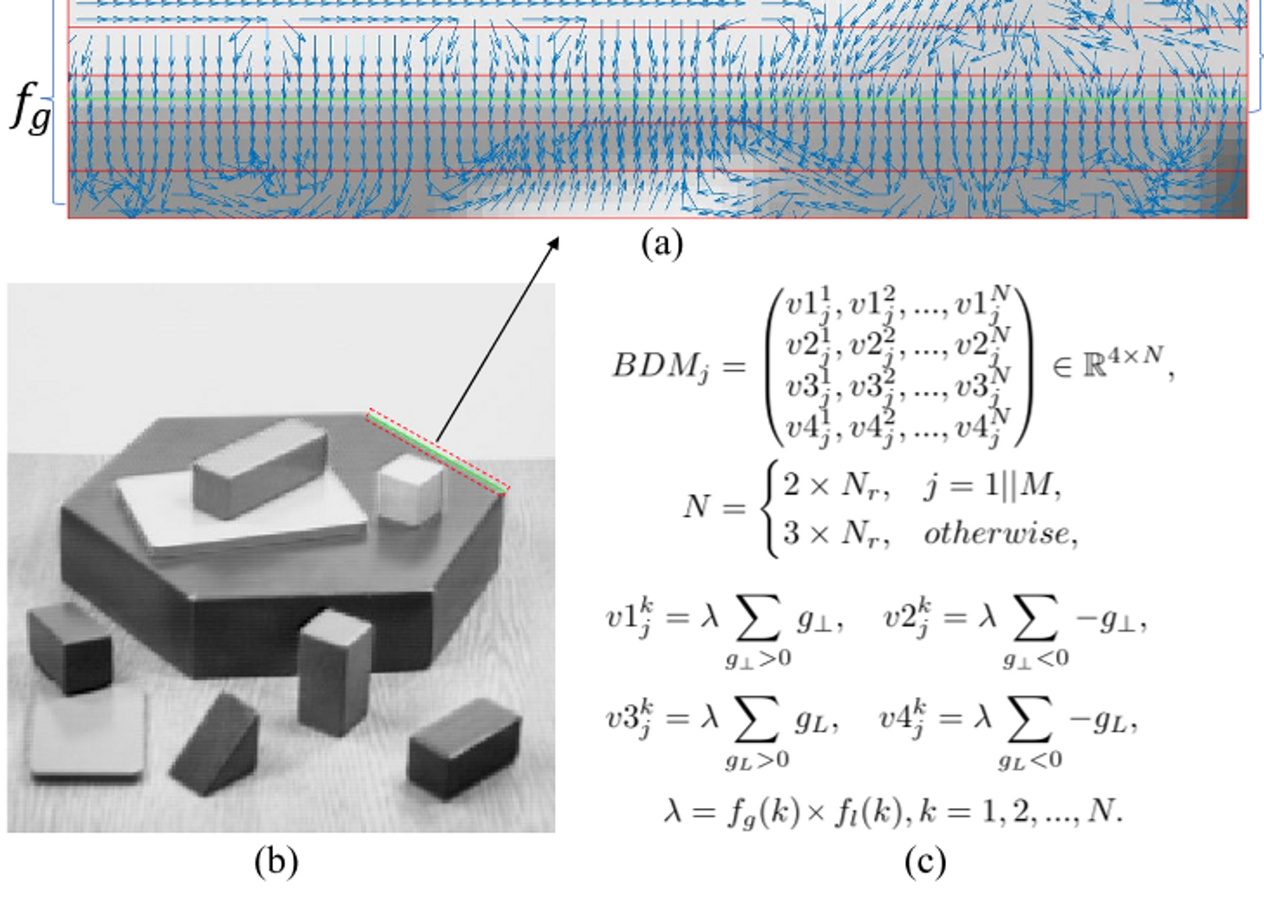
\includegraphics[width = 0.75\textwidth]{LBD.png}
  \caption{LBD方法示意图}
  \label{fig_LBD}
\end{figure}
基于统计的方法通过计算统计线相关的特征来描述线段,比如线梯度和线强度等。LBD是一种典型的基于统计描述方法。它采用了二进制编码,以紧凑的方式表示线段的局部特征,这使得它在快速匹配和检索任务中表现出色。LBD描述子具有旋转不变性,可以处理不同方向的线段,而无需进行旋转归一化,如图\ref{fig_LBD}所示。此外,它还具有尺度不变性,可适应不同尺度的线段。LBD描述子对抗噪声,适应线段形状的小变化,因此在实际应用中非常稳定。由于其二进制性质,LBD描述子可通过位运算进行高效匹配,这对于需要实时性能和大规模图像数据库的应用非常有帮助。LBD描述子关注线段周围的局部信息,从而能够有效地区分不同的线段模式。它通常用于线段匹配任务,如基于线段的目标识别、基于线段的姿态估计以及基于线段的视觉SLAM。因此,LBD描述子在计算机视觉领域扮演着重要的角色,为线段相关的应用提供了强大的工具。

\subsection{基于深度学习的方法}
基于深度学习的方法通过设计描述子网络来提取线段的描述子,其设计损失函数的理念是使得匹配的线段在描述空间中尽可能相近,使得不匹配的线段在描述空间中尽可能远离。根据网络推理的策略,可以将深度学习方法划分为基于线段支持区域的和不基于线段支持区域的两个种类。
\begin{enumerate}
  \item 基于线段支持区域的方法:在网络设计和训练中都用到线段周围的局部特征,并在此基础上进一步加入局部特征的描述子。
  \item 基于线段支持区域的方法:在网络设计和训练中都用到线段周围的局部特征,并在此基础上进一步加入局部特征的描述子。
\end{enumerate}

线段描述子提取方法总结如表\ref{tab_LineDes}所示。
\begin{table}[!ht]
  \centering
  \begin{tabular}{|c|c|c|c|c|}
  \hline
      类别 & 典型工作 & 优点 & 缺点 & 典型应用 \\ \hline
      Statistic-based & \makecell{LBD\cite{zhang2013efficient}\\MSLD\cite{wang2009msld}} & \parbox[c][13ex]{3.6cm}{一定程度抗干扰; 数学可解释} & \parbox[c][13ex]{3.6cm}{对低纹理场景敏感; 缺乏全局语义信息} & \makecell{视觉定位\\VSLAM} \\ \hline
      Structure-based & \makecell{NLD\cite{yammine2014novel}\\LS\cite{kim2010wide}} & \parbox[c][13ex]{3.6cm}{利用局部信息; 可以处理一些低纹理场景} & \parbox[c][13ex]{3.6cm}{要求线段共面; 丢失全局和语义信息} & 地图配准 \\ \hline
      Learning-based & \makecell{DLD\cite{lange2019dld}\\WLD\cite{lange2020wld}} & \parbox[c][13ex]{3.6cm}{端到端方法; 可以通过设计融合局部和全局信息} & \parbox[c][13ex]{3.6cm}{缺乏通用训练集和表示方法,且泛化性有待考证; GPU计算} & 场景解析和抽象 \\ \hline
  \end{tabular}
  \caption{线段描述子提取方法总结}
  \label{tab_LineDes}
\end{table}

\section{点线VIO框架}
\begin{figure}
  \centering
  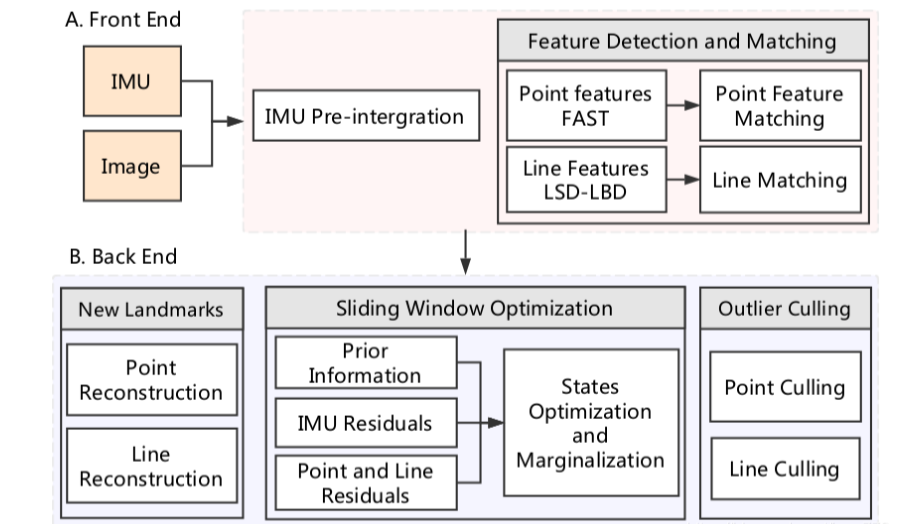
\includegraphics[width = 0.75\textwidth]{plvio.png}
  \caption{点线VIO框架图}
  \label{fig_PLVIO}
\end{figure}
点线VIO框架是一种用于移动机器人导航和定位的系统,它结合了图像和惯性传感器的数据,通过观察到的点和线段来实现相机位姿估计和轨迹场景重建。点线VIO框架具有三个模块,每个模块含有独立的节点执行不同的任务,如图\ref{fig_PLVIO}所示。
\begin{enumerate}
  \item 前端模块:前端模块中含有点特征和线特征的两个处理节点,主要负责图像数据的处理,包括提取视觉特征以及对提取的特征进行帧间匹配和追踪。这部分的关键任务是提供稳定高频率的图像特征跟踪结果,以便于后端进行进一步处理。
  \item 后端模块:后端节点负责通过融合来自前端的数据,执行位姿轨迹估计。根据处理方式的不同,后端节点算法分为基于滤波的方法和基于优化的方法。基于滤波的方法通过集成IMU测量来传播/预测状态,然后用视觉测量更新/修正最新的状态;基于优化的方法则直接通过最小化IMU测量残差和视觉重投影残差的联合非线性代价函数来获得最优估计。因此,基于优化的方法可以在不同的点上重复线性化状态向量,达到比基于滤波的方法更高的精度。
  \item 回环检测模块:回环检测节点负责检测机器人是否返回到先前访问过的位置,以纠正可能的定位漂移并提高定位的一致性。这通常涉及检测视觉特征的相似性,并在必要时进行回环修正,得到全局更优的估计结果。
\end{enumerate}

PL-VIO\cite{he2018pl}是第一个基于优化的点线特征联合VIO系统,此工作利用直线的标准正交表示,首次引入了IMU和点线特征的滑动窗口模型,并与点特征VIO框架进行了对比实验,如图\ref{fig_PLVIO_RMSE}所示,证明了线特征的加入对于位姿和轨迹估计的增益。
\begin{figure}
  \centering
  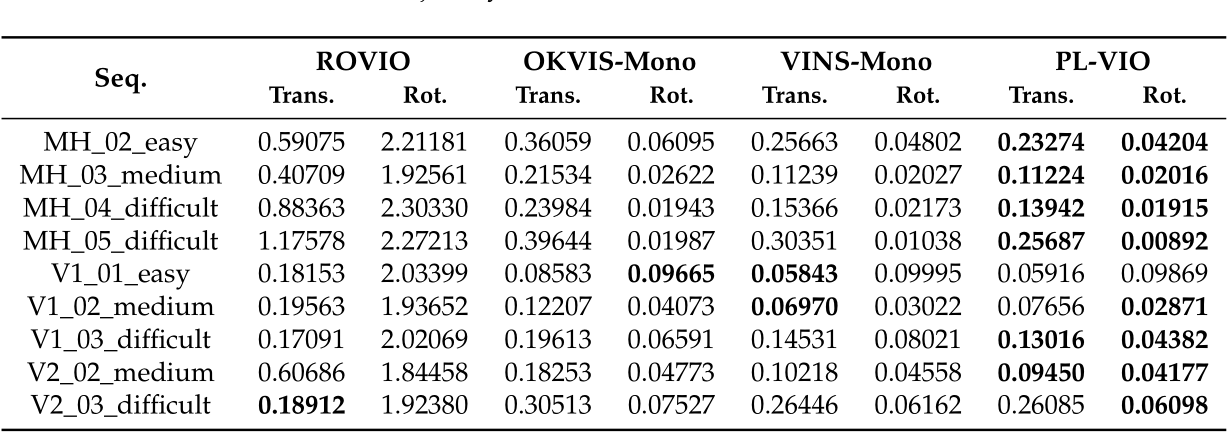
\includegraphics[width = 0.75\textwidth]{plvio-RMSE.png}
  \caption{PL-VIO精度测试结果(RMSE, Euroc@Intel Core i7-6700HQ CPU)}
  \label{fig_PLVIO_RMSE}
\end{figure}
对于轨迹平移和旋转的估计,PL-VIO几乎都取得了精度更高的效果,并且在难度较高的场景(对应特征更少、光照变化更剧烈的场景)中拥有更显著的优势。但是,由于线特征的加入,PL-VIO将耗费大量时间在线段的提取和参数化上,处理时间将恶化至点特征VIO的一倍以上,如图\ref{fig_PLVIO_TIME}。
\begin{figure}
  \centering
  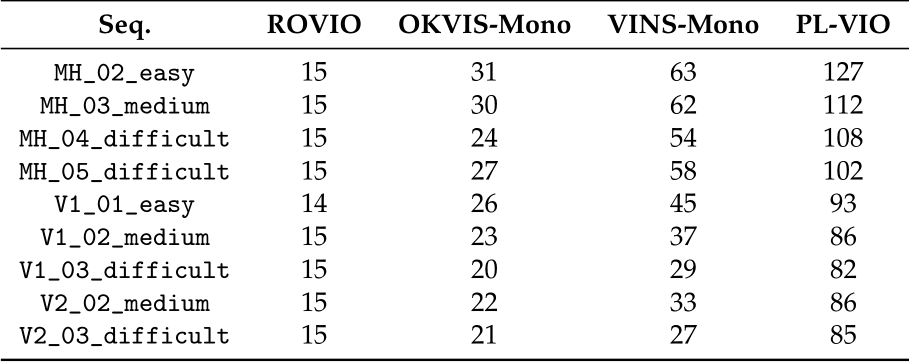
\includegraphics[width = 0.75\textwidth]{plvio-time.png}
  \caption{PL-VIO耗时测试结果(Euroc@Intel Core i7-6700HQ CPU)}
  \label{fig_PLVIO_TIME}
\end{figure}

PL-VINS\cite{fu2020pl}则针对线特征的耗时问题,对于LSD线段提取算法进行了速度优化,建立了第一个实时性单目点线VIO系统。由于LSD算法采用梯度聚合的方式,会提取到大量(超过500条)的短线,很难在下一帧中被匹配,这不仅浪费用于检测、描述和匹配的计算资源,也容易产生异常匹配导致性能恶化。PL-VINS基于这一观察构建了一个modified-LSD算法,一方面减少多尺度高斯滤波的金字塔层数,一方面对线段长度进行筛选,使得新算法运行速度可以达到LSD的三倍。

此外PL-VINS还基于VINS-Mono\cite{qin2018vins}的工作加入了线特征的前端处理器和后端优化器,构造了一个完整的点线VINS框架,相对VINS-Mono在Euroc数据集上取得了16\%的开环性能优化和12\%的闭环性能优化,如图\ref{fig_PLVINS_PREC}所示。
\begin{figure}
  \centering
  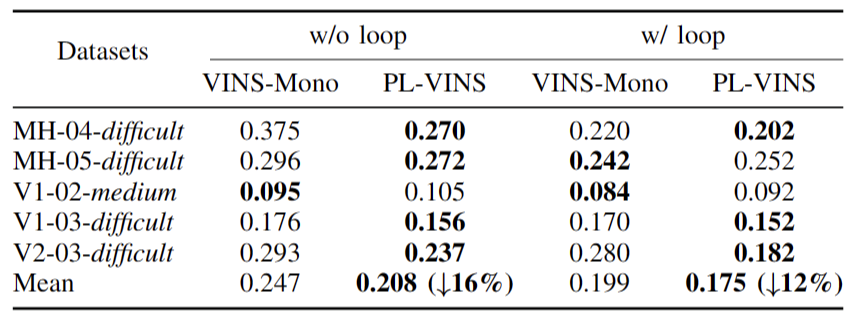
\includegraphics[width = 0.75\textwidth]{plvins-time.png}
  \caption{PL-VINS 精度测试结果}
  \label{fig_PLVINS_PREC}
\end{figure}
但是,PL-VINS框架中,使用的点特征提取(Shi-Tomasi角点检测)和匹配(KLT)算法,以及线特征提取(Modified-LSD)和匹配(KNN)算法均为非NN算法,在精度上还有较大的优化空间。现有的点线VIO框架并没有和基于神经网络的点线提取/匹配做良好的适配,导致这些方法难以在完整的VIO框架中得到应用。

\section{本章小结}
\label{outline}
基于以上的研究背景和前期调研结果,本实习课题以“实时点线联合VIO系统设计”为主要题目,并围绕以下两个问题展开:
\begin{enumerate}
  \item 针对现有点线联合VIO系统中缺少支持神经网络方法框架的问题,本课题基于PL-VINS框架建立了一个前端自定义的NN-PL-VINS框架,该框架支持用户自定义前端的点线提取和匹配方法,便于用户在不同场景下选择适合的方法以获得更佳的性能。
  \item 针对现有点线联合VIO系统中线检测和参数化耗时高的问题,本课题构造了一个点线联合推理网络SP-SOLD2,该网络可以通过一次推理得到点特征和线特征的提取结果以及对应的描述子,并且通过后处理的优化以及pipeline构建,此网络可以在NN-PL-VINS框架中取得相对现有工作更好的精度效果和更优的实时性能。
\end{enumerate}


% \section{引言的写法}

% 一篇学位论文的引言大致包含如下几个部分:
% 1、问题的提出;
% 2、选题背 景及意义;
% 3、文献综述;
% 4、研究方法;
% 5、论文结构安排。
% \begin{itemize}
%   \item 问题的提出:要清晰地阐述所要研究的问题“是什么”。
%     \footnote{选题时切记要有“问题意识”,不要选不是问题的问题来研究。}
%   \item 选题背景及意义:论述清楚为什么选择这个题目来研究,即阐述该研究对学科发展的贡献、对国计民生的理论与现实意义等。
%   \item 文献综述:对本研究主题范围内的文献进行详尽的综合述评,“述”的同时一定要有“评”,指出现有研究状态,仍存在哪些尚待解决的问题,讲出自己的研究有哪些探索性内容。
%   \item 研究方法:讲清论文所使用的学术研究方法。
%   \item 论文结构安排:介绍本论文的写作结构安排。
% \end{itemize}



% \section{正文的写法}

% 本部分是论文作者的研究内容,不能将他人研究成果不加区分地掺和进来。
% 已经在引言的文献综述部分讲过的内容,这里不需要再重复。
% 各章之间要存在有机联系,符合逻辑顺序。



% \section{结论的写法}

% 结论是对论文主要研究结果、论点的提炼与概括,应精炼、准确、完整,使读者看后能全面了解论文的意义、目的和工作内容。
% 结论是最终的、总体的结论,不是正文各章小结的简单重复。
% 结论应包括论文的核心观点,主要阐述作者的创造性工作及所取得的研究成果在本领域中的地位、作用和意义,交代研究工作的局限,提出未来工作的意见或建议。
% 同时,要严格区分自己取得的成果与指导教师及他人的学术成果。

% 在评价自己的研究工作成果时,要实事求是,除非有足够的证据表明自己的研究是“首次”、“领先”、“填补空白”的,否则应避免使用这些或类似词语。
